
%(BEGIN_QUESTION)
% Copyright 2014, Tony R. Kuphaldt, released under the Creative Commons Attribution License (v 1.0)
% This means you may do almost anything with this work of mine, so long as you give me proper credit

Write an equation that solves for the impedance of this series circuit.  The equation need not solve for the phase angle between voltage and current, but merely provide a scalar figure for impedance (in ohms):

$$\includegraphics[width=15.5cm]{i01074x01.eps}$$

\underbar{file i01074}
%(END_QUESTION)





%(BEGIN_ANSWER)

$Z_{total} = \sqrt{R^2 + (X_L - X_C)^2}$

%(END_ANSWER)





%(BEGIN_NOTES)

Ask your students why one of the reactance terms under the radicand is positive and the other is negative.  The way this equation is written, does it matter which term is negative?  As your students if we would obtain the same answer if it were written as $Z_{total} = \sqrt{R^2 + (X_C - X_L)^2}$ instead.  Challenge them to answer this question without using a calculator!

%INDEX% Electronics review: AC reactance and impedance

%(END_NOTES)


